% res_comparison.tex  -- written by Shivansh
\subsection{Comparison with the Sequential Baseline}
Table~\ref{tab:compare} and Fig.~\ref{fig:throughput} compare five design
points on a $4\times4$ product, including host data transfer. The compute
kernel alone is 5.4$\times$ faster than the baseline (12 vs.\ 65 cycles).
The Phase~I accelerator, however, is only 1.4$\times$ faster end to end,
because 48 of its 60 cycles move data one element at a time. This is
Amdahl's law in hardware: speeding up the 20\,\% compute part cannot help
the 80\,\% transfer part. Row-wide transfers cut this to 25 cycles.
Overlapping transfers with computation (ping-pong + result buffer) hides
them completely, giving 12.06 cycles per product, i.e.\ the 3N compute
bound. With both pipeline registers the design runs at 116~MHz and
completes a product every 121~ns (1.06~GOPS): 12.4$\times$ faster than the
baseline in wall-clock time.

\begin{table*}[t]
\centering
\caption{Design comparison for one $4\times4\times4$ product (host-visible). $f_{\max}$: post-route, Lattice ECP5-85F (nextpnr). Resources: Yosys \texttt{synth\_xilinx}, Xilinx 7-series.}
\label{tab:compare}
\begin{tabular}{@{}lrrrrrrrr@{}}
\toprule
\textbf{Design} & \textbf{cycles/product} & \textbf{$f_{\max}$ (MHz)} & \textbf{ns/product} & \textbf{GOPS} & \textbf{speed-up} & \textbf{DSP48} & \textbf{LUT} & \textbf{FF}\\
\midrule
Sequential, 1 MAC                 & 113   & 75.7  & 1493 & 0.09 & 1.0$\times$  & 1  & 82   & 40 \\
Phase~I systolic                  & 60    & 55.5  & 1081 & 0.12 & 1.4$\times$  & 16 & 1535 & 1064 \\
Phase~II, serial                  & 25    & 51.3  & 487  & 0.26 & 3.1$\times$  & 16 & 2534 & 1961 \\
Phase~II, overlapped              & 12.06 & 51.3  & 235  & 0.54 & 6.4$\times$  & 16 & 2534 & 1961 \\
Phase~II, overlapped + pipelined  & 14.06 & 116.4 & 121  & 1.06 & 12.4$\times$ & 16 & 3522 & 2284 \\
\bottomrule
\end{tabular}
\end{table*}

\begin{figure}[t]
\centering
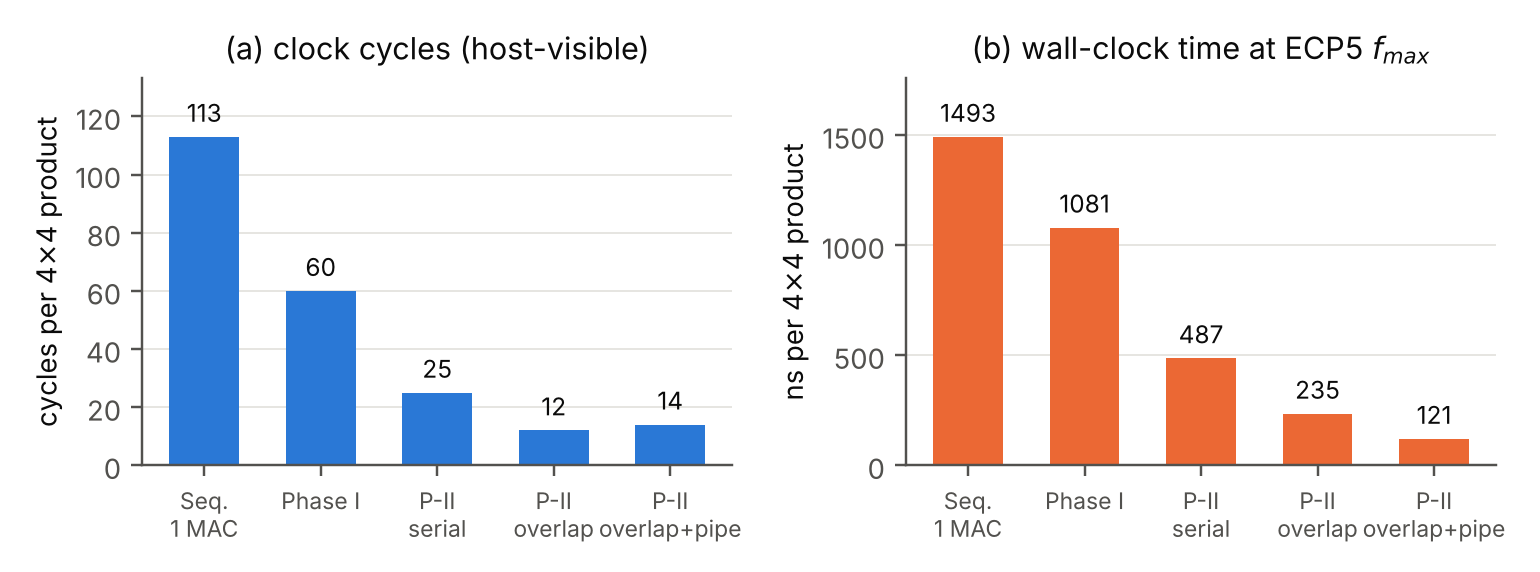
\includegraphics[width=\columnwidth]{fig_throughput.png}
\caption{Cycles and wall-clock time per $4\times4$ product for the five design points.}
\label{fig:throughput}
\end{figure}

The speed-up costs area: 16 DSP blocks instead of 1, and about 3.5\,k LUTs.
Per DSP block the systolic design is slightly less efficient than the
baseline (12.4$\times$ the throughput for 16$\times$ the multipliers),
which matches the 1/3 utilisation discussed above. Its advantage is that
the parallelism scales: at $N=16$ the same structure performs 83.6 MACs per
cycle, while a sequential design is fixed at one.
